\section{Results}
We analyzed short-term effects of \gls{RP} on accelerations, position, and Keplerian orbital elements. While position and orbital elements are ultimately relevant for precise orbit determination, examining the accelerations in different scenarios and along the orbit can explain why position and orbital elements changed. Additionally, the accelerations highlight differences between models of varying complexity.

To compare accelerations over one or multiple orbits, we used the \gls{RMSE}, which is defined as
\begin{align}
    \text{RMSE}(x, y) = \sqrt{\frac{1}{n}\sum_{i=1}^{n}\left(x_i - y_i\right)^2}.
\end{align}
The \gls{RMSE} describes the difference between two scalar timeseries and gives more weight to large deviations. These scalar timeseries can be the magnitude of accelerations or individual components. The \gls{rRMSE} is defined as
\begin{align}
    \text{rRMSE}(x, y) = \sqrt{\frac{\sum_{i=1}^{n}\left(x_i - y_i\right)^2}{\sum_{i=1}^{n} y_i^2}}
\end{align}
and useful to compare differences across orders of magnitude.

While the simulation evaluates accelerations in a global frame, the effect of accelerations on the orbit is best analyzed in a spacecraft-fixed coordinate system that is aligned with the orbital track. The RSW coordinate system is one such system, defined by the unit vectors~\cite{Vallado2013}
\begin{align}
    \vb R = \frac{\vb r}{\norm{\vb r}}, \quad
    \vb W = \frac{\vb r \times \vb v}{\norm{\vb r \times \vb v}},
    \quad \textrm{and} \quad \vb S = \vb W \times \vb R.
\end{align}
The radial component $\vb R$ is aligned with the planetocentric position vector $\vb r$. The cross-track component $\vb W$ is aligned with the angular momentum vector, or orbit plane normal, involving the linear velocity $\vb v$. The along-track component $\vb S$ completes the right-handed coordinate system. Note that $\vb S$ is generally not aligned with the velocity vector, only for circular orbits.





\subsection{Instantaneous reradiation}

First, we investigated the effect of instantaneous reradiation for the paneled target model. This increases the acceleration proportional to each panel's $C_a$, normal to the panel (cf. \cref{eq:brdf-reaction-specular-diffuse-instrerad}).

\begin{figure}[t]
    \centering
    \begin{subfigure}[c]{\linewidth}
        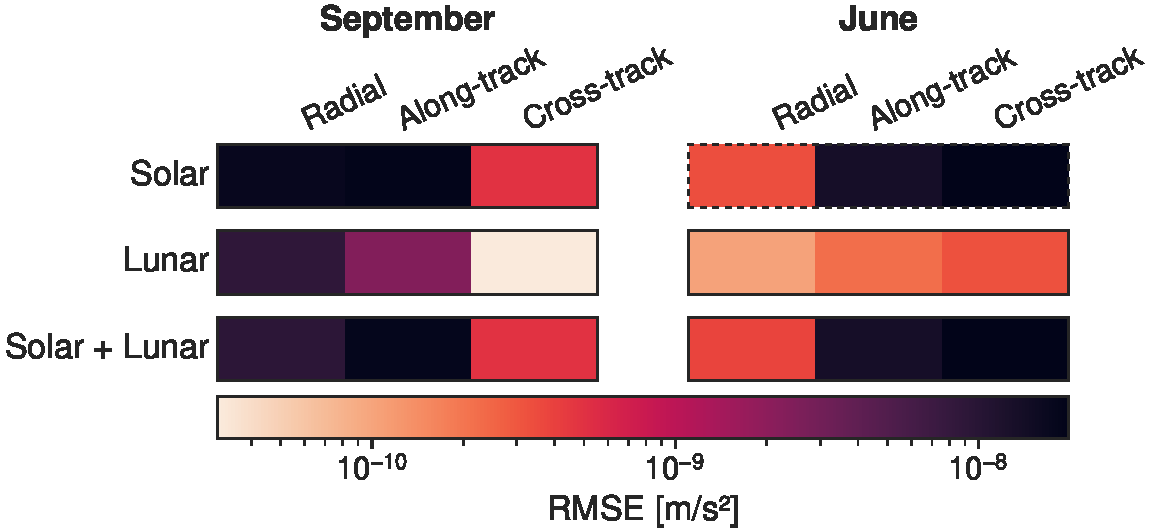
\includegraphics[width=\textwidth]{figures/plots/acc_reradiation_rms.pdf}
        \subcaption{Absolute}
     \end{subfigure}

     \bigskip

     \begin{subfigure}[c]{\linewidth}
        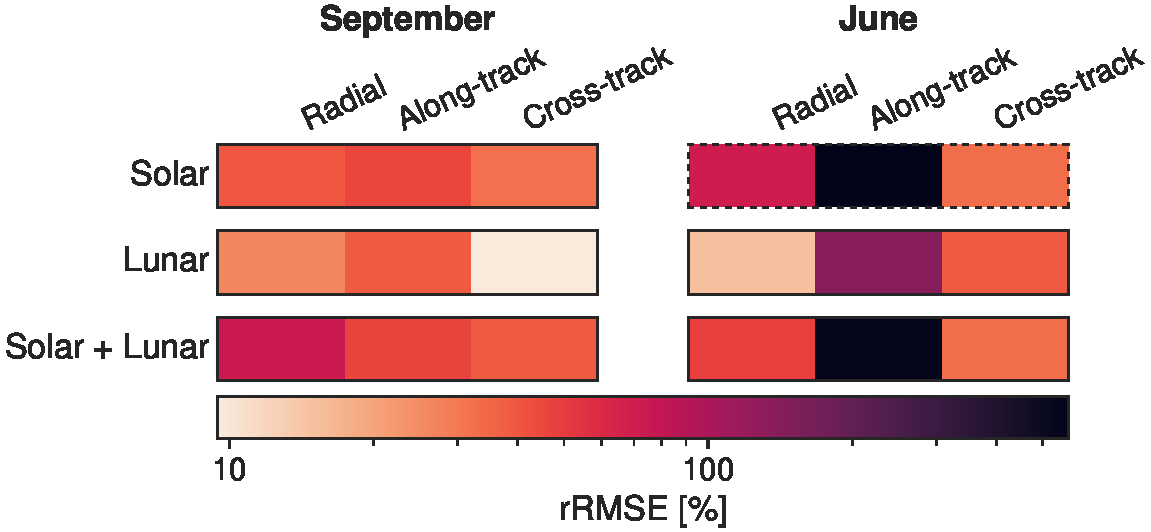
\includegraphics[width=\textwidth]{figures/plots/acc_reradiation_rrms.pdf}
        \subcaption{Relative}
     \end{subfigure}
    \caption{RMS differences of \gls{RP} accelerations over one orbit with and without instantaneous reradiation. The dashed box corresponds to \cref{fig:acc-reradiation}.}
    \label{fig:acc-reradiation-rms}
\end{figure}

\begin{figure}[t]
    \centering
    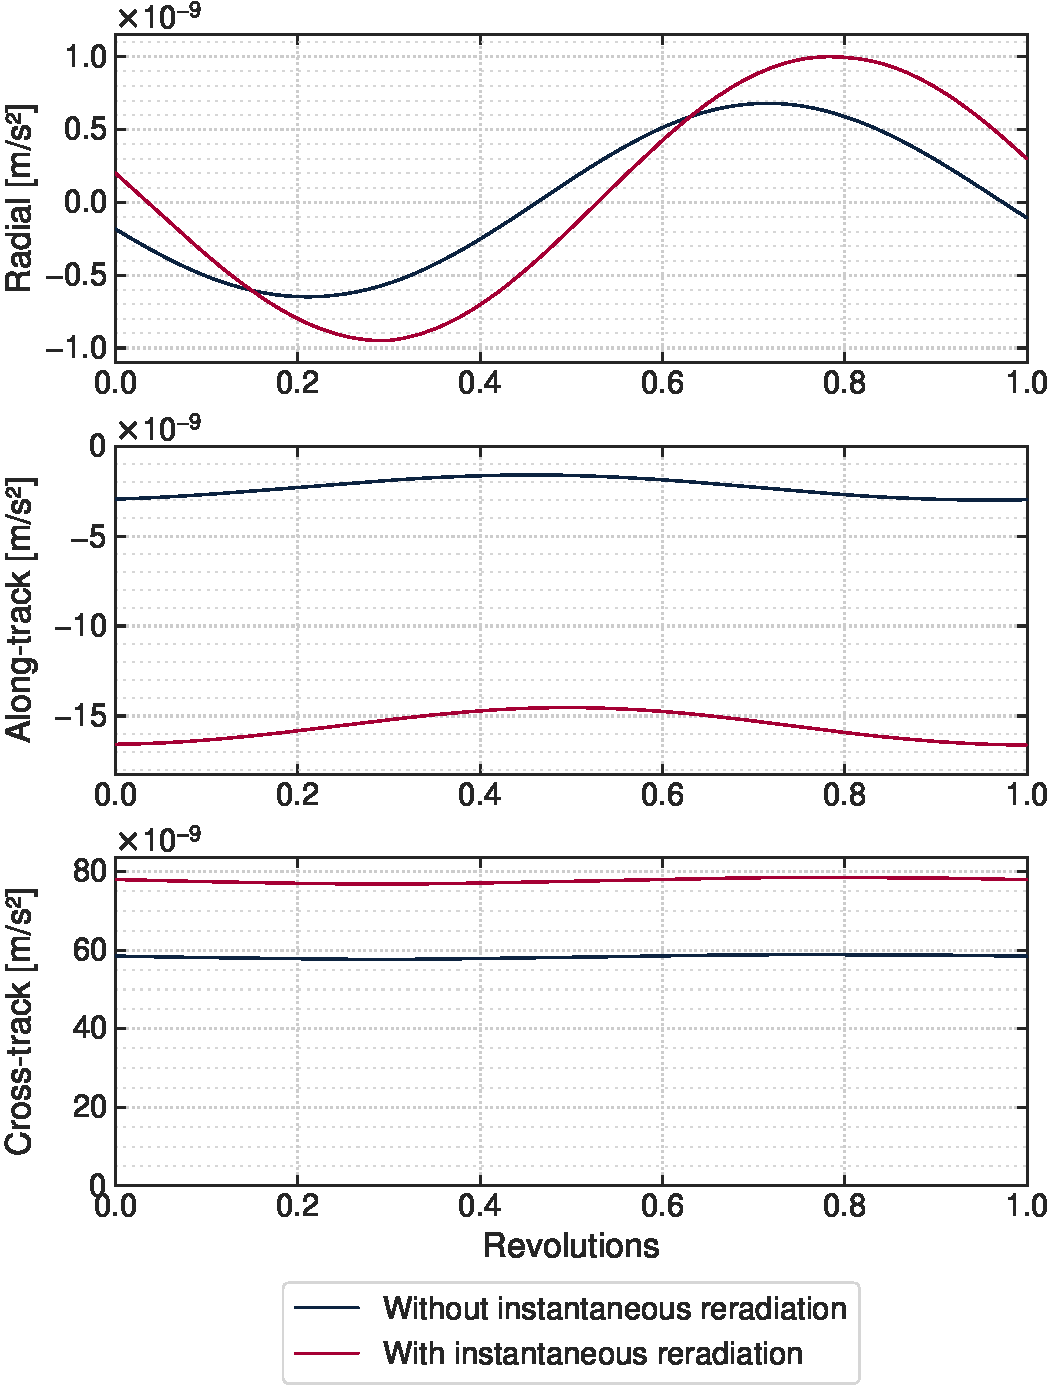
\includegraphics[width=\linewidth]{figures/plots/acc_reradiation_sun_jun.pdf}
    \caption{Solar \gls{RP} accelerations without and with instantaneous reradiation for June arc. There is a phase shift in the radial component and the along-track component increased by \qty{570}{\percent} \gls{RMSE}. Lunar contributions and the September arc are not sifnigicantly affected in shape.}
    \label{fig:acc-reradiation}
\end{figure}

\Cref{fig:acc-reradiation} shows the absolute and relative differences between accelerations without and with instantaneous reradiation. In absolute terms, the radial and along-track components are impacted most for the September arc, while the along-track and cross-track components experience the largest increase for the June arc (for both arcs, up to about \qty{1.9e-8}{\acc} \gls{RMSE}). The relative differences are more uniform (around \qty{40}{\percent} \gls{rRMSE}), but the along-track components of lunar and solar radiation in the June arc increase by \qty{140}{\percent} and \qty{570}{\percent} \gls{rRMSE}, respectively. In most cases, only the magnitude of accelerations changes but not their pattern.

\Cref{fig:acc-reradiation} shows the solar radiation of the June arc, the only of our simulations for which the pattern changed significantly. The phase of the radial acceleration is shifted by about \qty{10}{\percent} of the orbital period, which is not the case for the other two components or the acceleration due to lunar radiation. This arc also had the largest relative change in along-track acceleration as described above (highlighted in \cref{fig:acc-reradiation-rms}). This change is clearly visible as a constant offset of about \qty{13e9}{\acc}. 

The large changes seen in some cases are mostly due to the +SA panel, which is highly absorptive ($C_a = 0.90$) and large ($A = \qty{11.00}{\m\squared}$). For the June arc, the solar array is angled at \qty{45}{\degree} with equal components in the cross-track and along-track directions. Without instantaneous reradiation, no panel has a significant contribution to the along-track acceleration, so it is quite small at around \qty{2e-9}{\acc}. With instantaneous reradiation, each panel, and especially the solar array, exerts an acceleration parallel to its normal, which leads to the along-track increase witnessed for the June arc.

Since no reradiation due to spacecraft panels is physically unrealistic and the differences in magnitude are significant when instantaneous reradiation is added, we applied instantaneous reradiation for all other simulations. More sophisticated thermal models involving conduction and internal heat production would likely give more accurate results.




\subsection{Simulation setups}

Solar with/without
Lunar with/without
Albedo constant/dlam
LRO cannonball/paneled
with/without isntantaneous reradiation
Beta angle/arc

42 simulations

no knowledge of true RP accelerations
therefore, compare to baseline

cannonball with fixed Cr and paneled cannot directly be compared

Also use~\cite{Borderies1990} as reference for plots and discussion, especially about relation of acc and change in elements





\subsection{Accelerations}
thermal vs albedo

define along track, cross, radial

kink in cross-track SRP also seen in SELENE \cite{Kubooka1999}, search for explanation

Variation with orbital position and time of year (correlate with relative sun position and albedo map)

beta angle slightly less than 90 degrees leads to sinusoidal acceleration

show partial/full eclipse on time axis

absolute acceleration magnitude influenced by mass uncertainty
rp acceleration magnitude increases as mass decreases
17\% higher mass at start -> 17 \% lower acceleration magnitude

angle-based thermal behaves quite similar to albedo, but does not vanish in eclipse

cross track sign depends on sign of beta --> direction not super meaningful, also for orbital elements (e.g. change in lon asc node)

albedo likely overestimated by 25\% as described in \cref{subsec:lunar-albedo}

lunar RP dominated by thermal such that variations from DLAM1 are too small to have effect


\subsection{Change in final position}

Thermal in the range of a few meters ~\cite{Mazarico2011}

Thermal lunar radiation may cause an offset of 1-2 meters over an arclength of 2.5 days~\cite{Bauer2016}


\subsection{Change in orbital element}

compare wih Gauss perturbing equations (analytical solution to change of osculating elements based on accelerations), e.g. ~\cite[Sec.~3.2]{Lucchesi2006}

Keplerian state wrt ECLIPJ2000, not Moon frame!!




\subsection{Performance}
no special setup like cpu pinning or disabled hyperthreading for benchmarking
only on one setup
Performance may vary in other situations~\cite{Mytkowicz2009}
still, a good indication
also mention minimum

albedo model can increase computational demand by several hundred pct \cite{Nicholson2010}

